%======================================================================
% STAR System and Software User Manual (SSUM)
% Capstone Deliverable -- Spring 2026
% Self-contained single-file LaTeX source, 7-bit ASCII only.
% Compile: pdflatex STAR_System_and_Software_User_Manual.tex (run twice)
%======================================================================
\documentclass[11pt,letterpaper]{article}

%----------------------------------------------------------------------
% Packages (preamble paired with the STAR SDD for visual continuity)
%----------------------------------------------------------------------
\usepackage[margin=1in]{geometry}
\usepackage[T1]{fontenc}
\usepackage{lmodern}
\usepackage{xcolor}
\usepackage{graphicx}
\usepackage{booktabs}
\usepackage{array}
\usepackage{tabularx}
\usepackage{longtable}
\usepackage{enumitem}
\usepackage{parskip}
\usepackage{float}
\usepackage{caption}
\usepackage{fancyhdr}
\usepackage{titlesec}
\usepackage{amsmath}
\usepackage{amssymb}
\usepackage{siunitx}
\usepackage{listings}
\usepackage{tikz}
\usetikzlibrary{positioning, arrows.meta, shapes.geometric, fit, backgrounds}
\usepackage[colorlinks=true,
            linkcolor=blue!55!black,
            citecolor=blue!55!black,
            urlcolor=blue!55!black,
            pdftitle={STAR System and Software User Manual},
            pdfauthor={Cesar Magana (Team Locked Inc)},
            pdfsubject={STAR Capstone SSUM},
            pdfkeywords={STAR, ADA, operator manual, Grafana, Lichtblick,
                         Foxglove, ROS2, RX72N}]{hyperref}

%----------------------------------------------------------------------
% Status-label hyperlink macro (mirrors SDD)
% Use as: \statuslabel{IMPLEMENTED} / \statuslabel{STRETCH} /
%         \statuslabel{ARCHITECTED} / \statuslabel{STRETCH stub} /
%         \statuslabel{ARCHITECTED stubs}
% All occurrences hyperlink back to the legend at sec:status-legend.
%----------------------------------------------------------------------
\newcommand{\statuslabel}[1]{\hyperref[sec:status-legend]{[#1]}}

%----------------------------------------------------------------------
% Style
%----------------------------------------------------------------------
\pagestyle{fancy}
\fancyhf{}
\fancyhead[L]{\small STAR System and Software User Manual}
\fancyhead[R]{\small Spring 2026}
\fancyfoot[C]{\thepage}
\renewcommand{\headrulewidth}{0.4pt}
\renewcommand{\footrulewidth}{0.0pt}

\titleformat{\section}{\Large\bfseries}{\thesection}{0.75em}{}
\titleformat{\subsection}{\large\bfseries}{\thesubsection}{0.6em}{}
\titleformat{\subsubsection}{\normalsize\bfseries}{\thesubsubsection}{0.5em}{}
\titlespacing*{\section}{0pt}{14pt}{6pt}
\titlespacing*{\subsection}{0pt}{10pt}{4pt}

\definecolor{codegray}{gray}{0.45}
\definecolor{boxblue}{RGB}{230,240,255}
\definecolor{boxborder}{RGB}{70,110,170}
\definecolor{warnbg}{RGB}{255,240,220}
\definecolor{warnborder}{RGB}{200,120,30}

\lstdefinestyle{shellcmd}{
  frame=single,
  basicstyle=\small\ttfamily,
  breaklines=true,
  numbers=none,
  captionpos=b,
  keepspaces=true,
  showstringspaces=false,
  xleftmargin=0.8em,
  framexleftmargin=0.4em,
  aboveskip=0.4em,
  belowskip=0.4em
}

\sisetup{per-mode=symbol, detect-weight=true, detect-family=true}

%----------------------------------------------------------------------
% TikZ common styles (paired with SDD)
%----------------------------------------------------------------------
\tikzset{
  sddbox/.style = {rectangle, draw=boxborder, fill=boxblue, rounded corners,
                   minimum width=2.4cm, minimum height=0.9cm, align=center,
                   font=\small},
  sddlabel/.style = {font=\footnotesize\itshape},
  sddarrow/.style = {-Latex, thick, draw=boxborder}
}

%======================================================================
% Title Page
%======================================================================
\begin{document}
\thispagestyle{empty}

\begin{center}
\vspace*{1.0in}
{\Huge \bfseries System and Software User Manual}\\[0.35in]
{\LARGE STAR: Spatial Topography Accessibility Robot}\\[0.20in]
{\large Operator's Guide for Daily Use, Setup, and Maintenance}\\[0.8in]

\rule{4.5in}{0.8pt}\\[0.3in]

{\large \textbf{Team Locked Inc}}\\[0.15in]
\begin{tabular}{r l}
Cesar Magana        & Software \\
Brighton Sikarskie  & Software, Embedded Development, Schematic Design \\
Jeremie Hockey      & PCB Design and Layout \\
Michael Norton      & Mechanical Design \\
Shawn Ciaciura      & Schematic Review \\
Jared Bartz         & Schematic Review \\
\end{tabular}\\[0.4in]

{\large \textbf{Course}}\\[0.1in]
{\normalsize ESET 420 -- Senior Design II -- Dr. Lee Hudson}\\[0.4in]

{\large \textbf{Institution}}\\[0.1in]
{\normalsize Texas A\&M University}\\
{\normalsize Department of Electronic Systems Engineering Technology (ESET)}\\
{\normalsize ESET Senior Capstone, Spring 2026}\\[0.4in]

{\large \textbf{Advisors and Sponsors}}\\[0.1in]
{\normalsize Dr. Logan Porter -- Sponsor and Technical Advisor}\\[0.6in]

\rule{4.5in}{0.8pt}\\[0.2in]
{\large April 28, 2026}\\[0.15in]
{\small Version 1.0 -- Capstone Submission}

\end{center}
\clearpage

%======================================================================
% Front Matter
%======================================================================
\pagenumbering{roman}
\setcounter{page}{1}
\tableofcontents
\clearpage
\listoffigures
\listoftables
\clearpage

\pagenumbering{arabic}
\setcounter{page}{1}

%======================================================================
% 1. Scope
%======================================================================
\section{Scope}
\label{sec:scope}

\subsection{Purpose}
This manual is the operator-facing companion to the STAR Software
Description Document (SDD). The SDD explains HOW the STAR software is
designed and built; this manual explains HOW TO USE it. If a procedure
here is insufficient, consult the SDD for the underlying design, or
consult the source repository for authoritative detail.

\subsection{Audience}
The intended readers are:
\begin{itemize}[leftmargin=1.4em,itemsep=2pt]
\item Capstone reviewers validating that STAR can be operated by a
      non-developer through documented procedures.
\item Follow-on student teams inheriting the robot and needing to
      bring it up on new hardware or at a new site.
\item ADA facility auditors or building managers piloting STAR for a
      real compliance run.
\end{itemize}
Knowledge of Linux shells, SSH, and browser-based dashboards is
assumed; knowledge of ROS2 internals, C firmware, or protobuf is not.

\subsection{Out of Scope}
This manual does not cover software architecture, algorithm
derivations, data formats, testing strategy, or security design
decisions. Those live in the STAR SDD. Mechanical assembly, PCB
schematics, and BOM are covered in their own capstone deliverables.

\subsection{Status Label Legend}
\phantomsection
\label{sec:status-legend}
Throughout this document, three status labels identify how complete
each subsystem or feature is on the delivered system. Every body
occurrence of \texttt{[IMPLEMENTED]} / \texttt{[STRETCH]} /
\texttt{[ARCHITECTED]} elsewhere in this manual is a hyperlink back
to this legend.
\begin{itemize}[leftmargin=1.4em,itemsep=2pt]
\item \textbf{[IMPLEMENTED]} -- complete and exercised in daily use.
\item \textbf{[STRETCH]} -- partial implementation with scaffolding;
      fit for demonstration but not yet complete.
\item \textbf{[ARCHITECTED]} -- designed and specified but not coded.
\end{itemize}

%======================================================================
% 2. Referenced Documents
%======================================================================
\section{Referenced Documents}
\label{sec:refs}

\begin{itemize}[leftmargin=1.4em,itemsep=2pt]
\item STAR Software Description Document (companion capstone
      deliverable, \texttt{final\_docs/software\_description\_document/}).
\item \texttt{docs/ARCHITECTURE.md} -- end-to-end operations stack
      topology (Pi5, Tailscale, k3s, Cloudflare).
\item \texttt{infra/README.md} -- Pi5-side system files, Caddy
      configuration, systemd units, and fresh-Pi5 install procedure.
\item \texttt{docs/PI\_DEPLOYMENT.md} -- ROS2 Jazzy workstation and
      Pi5 provisioning.
\item \texttt{scripts/flash-rx72n.sh} -- RX72N firmware flashing
      helper.
\item \texttt{monitoring/grafana-star-dashboard.json} -- Grafana
      dashboard definition used by the operator cockpit.
\item \texttt{star-ros2/src/star\_simple\_bridge/} -- MVP ROS2 bridge
      that serves Prometheus metrics and map images.
\item \texttt{star-ros2/src/star\_bringup/foxglove/star-default.json}
      -- default Foxglove / Lichtblick layout.
\item U.S. Department of Justice, \textit{2010 ADA Standards for
      Accessible Design}, Section 405.2 (Ramp Running Slope).
      \url{https://www.access-board.gov/ada/chapter/ch04/}
\item Open Navigation LLC, Nav2 navigation framework documentation.
      \url{https://docs.nav2.org/}
\item Lichtblick, \texttt{lichtblick-suite/lichtblick} static web
      bundle (Foxglove Studio fork).
      \url{https://github.com/lichtblick-suite/lichtblick}
\item Open Robotics, ROS 2 Jazzy Jalisco (LTS, May 2024 -- May
      2029, Ubuntu 24.04). \url{https://docs.ros.org/en/jazzy/}
\end{itemize}

%======================================================================
% 3. Software Summary
%======================================================================
\section{Software Summary}
\label{sec:summary}

\subsection{What STAR Does}
STAR is an autonomous indoor mobile robot that performs ADA Title III
compliance audits. The operator drives or dispatches the robot into a
building; the robot maps the space, measures geometric features (ramp
slope, path width, trip hazards), and produces a structured compliance
report. All of the control software runs on a Raspberry Pi 5 on the
robot; a second microcontroller (Renesas RX72N) performs real-time
motor control. The operator interacts with STAR through web-based
dashboards -- primarily Grafana for control and Lichtblick (or
Foxglove) for 3D visualization.

\subsection{Operator-Visible Software Inventory}
Table~\ref{tab:inventory} summarizes what the operator actually sees
and uses. Everything underneath is described in the SDD.

\begin{table}[H]
\centering
\caption{Operator-visible software inventory.}
\label{tab:inventory}
\small
\begin{tabularx}{\linewidth}{l l X}
\toprule
\textbf{Component} & \textbf{Where} & \textbf{What it does for the operator} \\
\midrule
Grafana dashboard       & k3s cluster / browser
    & Primary cockpit. Live telemetry, autonomy toggle, e-stop,
      speed, SLAM controls. \statuslabel{IMPLEMENTED} \\
Lichtblick web app      & k3s cluster / browser
    & 3D visualization of LiDAR, map, odometry, and TF tree.
      Foxglove-compatible. \statuslabel{IMPLEMENTED} \\
Foxglove Studio desktop & Laptop (tailnet)
    & Power-user alternative to Lichtblick, same layout file.
      \statuslabel{IMPLEMENTED} \\
\texttt{star\_cockpit\_api} & Pi5 \texttt{:9102}
    & HTTP API backing the Grafana cockpit toggles.
      \statuslabel{IMPLEMENTED} \\
\texttt{star\_simple\_bridge} & Pi5 \texttt{:9101}
    & ROS2 serial bridge to RX72N, Prometheus metrics, map image
      server. \statuslabel{IMPLEMENTED} \\
Caddy (Pi5-side)        & Pi5 \texttt{:443}
    & Local-CA TLS front for \texttt{star.local}. \statuslabel{IMPLEMENTED} \\
\texttt{star-slam-mvp.service} & Pi5 systemd
    & Autostarts the SLAM MVP node set on boot; safe MANUAL state.
      \statuslabel{IMPLEMENTED} \\
RX72N firmware          & On-board MCU
    & Closed-loop motor control, encoder and IMU decoding.
      \statuslabel{IMPLEMENTED} \\
\texttt{flash-rx72n.sh}  & Workstation
    & One-shot firmware flashing helper. \statuslabel{IMPLEMENTED} \\
\bottomrule
\end{tabularx}
\end{table}

\subsection{Operator Connection Topology}
Figure~\ref{fig:topology} summarizes how an operator in a browser
reaches the robot. The Pi5 is on a Tailscale mesh (IP
\texttt{100.64.0.6}); a k3s homelab cluster hosts Grafana and
Lichtblick; a public Caddy instance on the homelab fronts both for
Cloudflare TLS.

\begin{figure}[H]
\centering
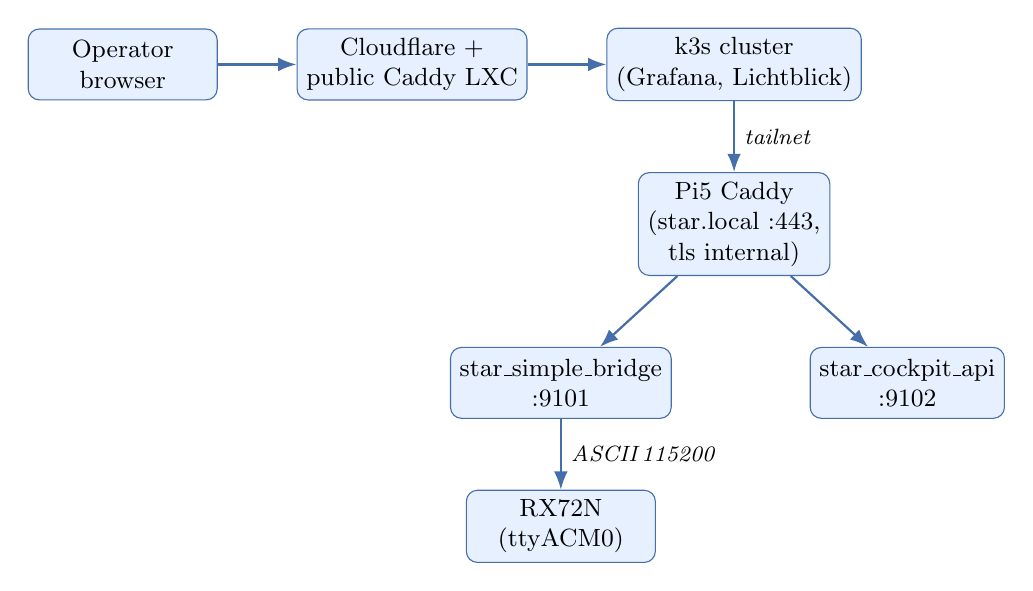
\begin{tikzpicture}[node distance=0.9cm and 1.0cm]
\node[sddbox] (br)  {Operator\\browser};
\node[sddbox, right=of br] (cf) {Cloudflare +\\public Caddy LXC};
\node[sddbox, right=of cf] (k3) {k3s cluster\\(Grafana, Lichtblick)};
\node[sddbox, below=of k3] (ca) {Pi5 Caddy\\(star.local :443,\\tls internal)};
\node[sddbox, below=of ca, xshift=-2.2cm] (sb) {star\_simple\_bridge\\:9101};
\node[sddbox, below=of ca, xshift=2.2cm]  (co) {star\_cockpit\_api\\:9102};
\node[sddbox, below=of sb] (rx) {RX72N\\(ttyACM0)};

\draw[sddarrow] (br) -- (cf);
\draw[sddarrow] (cf) -- (k3);
\draw[sddarrow] (k3) -- (ca) node[midway,right,sddlabel]{tailnet};
\draw[sddarrow] (ca) -- (sb);
\draw[sddarrow] (ca) -- (co);
\draw[sddarrow] (sb) -- (rx) node[midway,right,sddlabel]{ASCII\,115200};
\end{tikzpicture}
\caption{Operator connection topology. The Pi5 appears to the operator
as \texttt{star.local}; Grafana and Lichtblick live in a homelab k3s
cluster that is also on the Tailscale mesh.}
\label{fig:topology}
\end{figure}

%======================================================================
% 4. Installation and First-Time Setup
%======================================================================
\section{Installation and First-Time Setup}
\label{sec:install}

This section covers procedures you perform once per site or robot. For
daily operation see Section~\ref{sec:daily}.

\subsection{Prerequisites}
\begin{itemize}[leftmargin=1.4em,itemsep=2pt]
\item STAR robot with charged battery pack, RPLiDAR C1, BNO055 IMU,
      and four DRV8263H-driven motors.
\item Raspberry Pi 5 running Ubuntu 24.04 with ROS2 Jazzy installed
      per \texttt{docs/PI\_DEPLOYMENT.md}.
\item Operator laptop with a modern browser and a Tailscale client
      enrolled in the same tailnet as the Pi5.
\item USB-C power for the workstation, Renesas E2 Lite debugger for
      initial firmware flashing, and a USB-A to micro-USB cable for
      SCI boot-mode fallback.
\end{itemize}

\subsection{Provisioning the Pi5}
Follow \texttt{docs/PI\_DEPLOYMENT.md} end-to-end. At a minimum:
\begin{enumerate}[leftmargin=1.4em,itemsep=2pt]
\item Install ROS2 Jazzy from the OSRF apt repository and source
      \texttt{/opt/ros/jazzy/setup.bash}.
\item Install the STAR udev rules for \texttt{/dev/star-mcu} and
      \texttt{/dev/star-lidar} so device paths are stable across
      reboots.
\item Enroll the Pi5 in Tailscale and confirm its address resolves
      to \texttt{100.64.0.6} (or whichever tailnet address is
      documented for your team).
\item Build the ROS2 workspace with \texttt{./build-ros2.sh}.
\end{enumerate}

\subsection{Installing Pi5 Infrastructure Files}
Refer to \texttt{infra/README.md}. Copy the system files into place on
a fresh Pi5:
\begin{lstlisting}[style=shellcmd]
# From the repository root on the Pi5
sudo cp infra/pi5/opt/star_cockpit_api/server.py \
        /opt/star_cockpit_api/
sudo chmod +x /opt/star_cockpit_api/server.py

sudo cp infra/pi5/etc/caddy/Caddyfile /etc/caddy/Caddyfile
sudo cp infra/pi5/etc/systemd/system/*.service \
        /etc/systemd/system/

# Install Caddy (arm64)
sudo curl -fsSL -o /usr/local/bin/caddy \
  "https://caddyserver.com/api/download?os=linux&arch=arm64"
sudo chmod +x /usr/local/bin/caddy

sudo systemctl daemon-reload
sudo systemctl enable --now caddy.service
sudo systemctl enable --now star-cockpit-api.service
sudo systemctl enable --now star-slam-mvp.service
\end{lstlisting}

After this, rebooting the Pi5 brings up the complete operator stack
automatically: Caddy on port 443, cockpit API on 9102,
\texttt{star\_simple\_bridge} on 9101, and the SLAM MVP ROS2 node
set in MANUAL mode with the emergency stop cleared.

\subsection{Flashing the RX72N Firmware}
Two flashing methods are supported by \texttt{scripts/flash-rx72n.sh}:

\textbf{E2 Lite (default, recommended for lab work):}
\begin{itemize}[leftmargin=1.4em,itemsep=2pt]
\item SW4 Pin1 = OFF, Pin2 = OFF (Single Chip Mode).
\item Board powered externally.
\item FINE interface at \qty{250}{\kilo\bit\per\second}.
\item \qty{1}{\mega\bit\per\second} FINE causes framing errors on
      the STAR PCB and must not be used.
\end{itemize}

\textbf{SCI Boot Mode (field fallback via on-board USB-UART):}
\begin{itemize}[leftmargin=1.4em,itemsep=2pt]
\item SW4 Pin1 = ON, Pin2 = OFF.
\item Power-cycle the board AFTER setting the switches.
\item After a successful flash, return SW4 Pin1 = OFF and power-cycle
      again to run the new image.
\end{itemize}

On Apple Silicon and ARM Linux workstations, Renesas only ships
\texttt{rfp-cli} as an x86\_64 binary. The
\texttt{flash-rx72n.sh} helper detects an aarch64 host and
launches \texttt{rfp-cli} through \texttt{box64} when present, which
avoids a known SIGSEGV that the kernel's binfmt + qemu-user fallback
hits during \texttt{rfp-cli} startup. Install \texttt{box64} once
on aarch64 hosts; x86\_64 hosts run \texttt{rfp-cli} natively.

\begin{lstlisting}[style=shellcmd]
# Build a release image and flash via E2 Lite
make build-rx72n-release
./scripts/flash-rx72n.sh \
    star-rx72n-firmware/build/release/star-rx72n.mot

# Fallback over on-board USB-UART (SCI Boot Mode)
./scripts/flash-rx72n.sh \
    star-rx72n-firmware/build/release/star-rx72n.mot \
    sci /dev/ttyACM0
\end{lstlisting}

\subsection{Grafana and Lichtblick Deployment}
Grafana, Prometheus, and Lichtblick are deployed as k3s workloads on
the homelab cluster (Tailscale address \texttt{100.64.0.1}). The
Grafana dashboard is pushed into running Grafana via its HTTP API, so
the authoritative source of truth is the JSON file at
\texttt{monitoring/grafana-star-dashboard.json}. After any edit,
re-pushing the dashboard is a one-step operation the cluster admin
performs out of band.

The Grafana dashboard iframes the STAR map served by
\texttt{star\_simple\_bridge} at
\texttt{https://star.local/map.png}, which requires the operator's
browser to trust the Pi5 Caddy's local CA. See
\texttt{docs/ARCHITECTURE.md} for the one-time browser trust-store
step.

\subsection{Optional: Local Lichtblick Web Bundle}
The public Lichtblick URL is the primary 3D viz path. For
demos in places without reliable internet (the senior-design
showcase floor in particular), the script
\texttt{scripts/setup-lichtblick-web.sh} downloads the
\texttt{lichtblick-suite/lichtblick} static web bundle to
\texttt{/opt/star-lichtblick-web} so the Pi5 can serve it
locally over the on-board AP at
\texttt{http://192.168.50.1:8081}. The Pi5 default layout at
\texttt{star-ros2/src/star\_bringup/foxglove/star-default.json}
is preserved on every run. \statuslabel{IMPLEMENTED}.
\begin{lstlisting}[style=shellcmd]
# One-time, with the Pi5 on the internet
sudo ./scripts/setup-lichtblick-web.sh
# Default install pins lichtblick v1.24.3.
\end{lstlisting}

\subsection{Bring-Up Helper: \texttt{slam-mvp.sh}}
\texttt{scripts/slam-mvp.sh} is the canonical one-command bring-up
that \texttt{star-slam-mvp.service} runs on boot. It is also useful
on a developer workstation. The four subcommands:
\begin{itemize}[leftmargin=1.4em,itemsep=2pt]
\item \texttt{slam-mvp.sh start [--mcu /dev/star-mcu]
      [--lidar /dev/star-lidar]} -- launches each ROS2 node in the
      MVP set as a separate background process with its own log
      file under \texttt{/tmp/slam-mvp-logs/}. PIDs land in
      \texttt{/tmp/slam-mvp.pids}.
\item \texttt{slam-mvp.sh status} -- reports which PIDs are still
      alive and which logs were written.
\item \texttt{slam-mvp.sh stop} -- sends SIGTERM, then SIGKILL after
      a grace window.
\item \texttt{slam-mvp.sh logs <node>} -- tails the per-node log
      file (e.g. \texttt{slam-mvp.sh logs simple\_bridge}).
\end{itemize}
If \texttt{/dev/star-mcu} is missing at start time -- which happens
when the E2 Lite holds the RX72N in reset during power-up ordering
and starves the Cypress USB-UART -- the script automatically cycles
the E2 Lite USB device (vendor \texttt{045b}, product
\texttt{82a0}) to release reset. The MCU enumerates within roughly
one second.

\subsection{Verifying the Install}
From the operator's browser on the tailnet, confirm each surface is
reachable:
\begin{itemize}[leftmargin=1.4em,itemsep=2pt]
\item \texttt{https://star.local/} -- Pi5 Caddy serves
      \texttt{star\_simple\_bridge}; \texttt{/map.png} returns an
      image (or a 404 until SLAM has produced a map).
\item \texttt{https://star.local/api/state} -- cockpit API returns
      \texttt{\{autonomy, estop, speed, slam\}} JSON.
\item Grafana URL (deployed through public Caddy + Cloudflare) --
      the STAR dashboard loads and panels populate within seconds.
\item Lichtblick URL (deployed through public Caddy + Cloudflare) --
      the default layout loads; click "Open Connection" and enter
      \texttt{ws://100.64.0.6:8765} to attach to the foxglove
      bridge on the robot.
\end{itemize}

%======================================================================
% 5. Daily Operation
%======================================================================
\section{Daily Operation Procedures}
\label{sec:daily}

\subsection{Power-On Sequence}
\begin{enumerate}[leftmargin=1.4em,itemsep=2pt]
\item Verify the battery pack is seated and the main breaker is OFF.
\item Flip the main breaker ON. The Pi5 boots; the RX72N status LED
      begins its breathing pattern within a second.
\item Wait approximately 30 seconds for ROS2, Caddy, and the
      cockpit API to come up (driven by
      \texttt{star-slam-mvp.service}).
\item Confirm Tailscale has assigned the Pi5 its tailnet address.
      (The Pi5 side has a \qty{8}{\second} USB-enumeration delay
      before the SLAM MVP script starts.)
\item The robot is now in MANUAL mode with the emergency stop
      cleared. It will not move until you command it.
\end{enumerate}

\subsection{Opening the Cockpit}
Open two browser tabs from the operator laptop:
\begin{enumerate}[leftmargin=1.4em,itemsep=2pt]
\item The public Grafana URL (see
      Section~\ref{sec:install}). The STAR dashboard has control
      panels for autonomy, e-stop, speed, and SLAM, plus live
      telemetry gauges.
\item The public Lichtblick URL. The default layout loads the
      3D scene, LiDAR, map, stereo point cloud, and IMU plots.
      In "Open Connection", enter \texttt{ws://100.64.0.6:8765}.
\end{enumerate}

\subsection{Granting the Browser Trust for \texttt{star.local}}
The Grafana dashboard loads map images directly from
\texttt{https://star.local/map.png}. This URL is served by the Pi5's
Caddy using a local CA. Install that CA on the operator laptop one
time (per \texttt{docs/ARCHITECTURE.md}), otherwise the map panel
will show a broken-image placeholder.

\subsection{Teleoperation (MANUAL mode)}
In MANUAL mode the robot follows velocity commands from the Grafana
cockpit or from a publisher on \texttt{/cmd\_vel}. Two input options:
\begin{itemize}[leftmargin=1.4em,itemsep=2pt]
\item \textbf{Grafana speed panel:} POST to
      \texttt{/api/speed} with a scalar in $[0, 1]$, then POST
      linear/angular velocity deltas to \texttt{/api/cmd\_vel}.
\item \textbf{USB gamepad} (at the workstation): left stick Y axis
      commands linear velocity (inverted), left stick X axis
      commands angular velocity; deadzone is 0.1; commands publish
      at \qty{50}{\hertz}.
\end{itemize}
The \texttt{star\_safety\_monitor} enforces a linear ceiling of
\qty{1.0}{\meter\per\second} and an angular ceiling of
\qty{2.0}{\radian\per\second}. Commands outside this envelope are
clamped.

\subsection{Switching to AUTONOMY}
From the Grafana cockpit, click the AUTONOMY toggle. This sends
\texttt{POST /api/autonomy/toggle} to the cockpit API, which flips
the latched \texttt{/star/autonomy\_enable} topic. When AUTONOMY is
on, the supervisor forwards Nav2's \texttt{/nav2/cmd\_vel} to the
gated \texttt{/cmd\_vel\_out} that
\texttt{star\_simple\_bridge} consumes; operator teleop is ignored.

To give a Nav2 goal, click a target on the Lichtblick 3D panel
configured to publish to \texttt{/goal\_pose}. Nav2 plans and
executes, publishing status back to the topic tree.

\subsection{Running SLAM}
If SLAM is not already active:
\begin{enumerate}[leftmargin=1.4em,itemsep=2pt]
\item Click the SLAM START toggle in Grafana (POSTs to
      \texttt{/api/slam/start}). The cockpit API activates the
      \texttt{/slam\_toolbox} lifecycle node.
\item Drive the robot slowly through the space. The Lichtblick map
      panel fills in as scans accumulate. A separate SLAM map can be
      viewed directly at
      \texttt{https://star.local/map.png}.
\item When finished, click SLAM STOP to deactivate the node. To
      reset the map, send
      \texttt{POST /map/reset?confirm=yes} to
      \texttt{https://star.local/map/reset} on
      \texttt{star\_simple\_bridge}.
\end{enumerate}

\subsection{Running a Compliance Audit}
Compliance nodes (Section~\ref{sec:topics}) publish check results on
the \texttt{/compliance/*} topics whenever SLAM is active and the
robot is moving. The ramp-slope check is \statuslabel{IMPLEMENTED};
other checks are \statuslabel{STRETCH} or \statuslabel{ARCHITECTED}
per the SDD traceability matrix. The
report generator in
\texttt{final\_capstone/compliance-engine/star\_compliance/report/}
produces a PDF audit report at the end of a run; copy it off the Pi5
over SCP.

\subsection{Graceful Shutdown}
\begin{enumerate}[leftmargin=1.4em,itemsep=2pt]
\item From Grafana, clear AUTONOMY (back to MANUAL) and optionally
      SLAM STOP.
\item SSH to the Pi5 and run \texttt{sudo systemctl stop
      star-slam-mvp.service} to bring down ROS2 nodes gracefully.
\item Run \texttt{sudo shutdown -h now} on the Pi5.
\item Wait for the Pi5 power LED to extinguish, then flip the main
      breaker OFF.
\end{enumerate}

%======================================================================
% 6. Dashboard Reference
%======================================================================
\section{Dashboard Reference}
\label{sec:dashboards}

\subsection{Grafana Cockpit}
The committed dashboard is
\texttt{monitoring/grafana-star-dashboard.json}. It contains row
groups for SLAM map, motors, safety, sensors, and SLAM diagnostics.
Key widgets the operator uses:
\begin{itemize}[leftmargin=1.4em,itemsep=2pt]
\item \textbf{Map panel:} iframe-style HTML rendering of
      \texttt{https://star.local/map.png}. Auto-refreshes on the
      Grafana time-range tick.
\item \textbf{Motor gauges:} per-wheel velocity in
      \unit{\meter\per\second} (metric
      \texttt{star\_motor\_velocity\_mps\{wheel=...\}}).
\item \textbf{E-stop button and indicator:} POST
      \texttt{/api/estop/toggle}. The indicator gauge reflects the
      latched \texttt{/star/estop} topic.
\item \textbf{Autonomy toggle:} POST
      \texttt{/api/autonomy/toggle}.
\item \textbf{Speed slider:} POST \texttt{/api/speed} with a scalar
      in $[0, 1]$ that becomes \texttt{/star/speed\_scale}.
\item \textbf{SLAM start/stop buttons:} POST
      \texttt{/api/slam/start} or \texttt{/api/slam/stop}.
\end{itemize}
Grafana's minimum refresh interval is configured to
\qty{1}{\second} via the \texttt{GF\_DASHBOARDS\_MIN\_REFRESH\_INTERVAL}
environment variable on the Grafana pod.

\subsection{Lichtblick Layout}
The default layout
\texttt{star-ros2/src/star\_bringup/foxglove/star-default.json}
wires the following topics into Lichtblick's 3D panel:
\begin{itemize}[leftmargin=1.4em,itemsep=2pt]
\item \texttt{/scan} -- RPLiDAR C1 scan (visible, green, 5 px).
\item \texttt{/map} -- occupancy grid from \texttt{slam\_toolbox}.
\item \texttt{/cloud\_map} -- 3D point cloud, height-colored, 6 px.
\item \texttt{/octomap\_occupied\_space} -- Octomap (hidden by
      default; enable for obstacle review).
\item \texttt{/stereo/points2} -- stereo-camera point cloud, 4 px,
      rainbow-colored.
\item \texttt{/tf} -- transform tree.
\item \texttt{/odometry/filtered} -- EKF odometry, arrow marker.
\item \texttt{/odom/unfiltered} -- raw wheel odometry, arrow marker.
\end{itemize}

\subsubsection*{Foxglove Gauge Mirror Topics}
\texttt{sensor\_msgs/Imu} and the wheel \texttt{Float32MultiArray}
topics carry nested fields that Foxglove Gauge panels cannot read
directly. \texttt{star\_simple\_bridge} mirrors the relevant scalars
into single-valued \texttt{std\_msgs/Float32} topics so each Gauge
binds to one topic. These are the topics to use when building
custom Foxglove panels:
\begin{table}[H]
\centering
\caption{Scalar telemetry topics for Foxglove Gauge panels.}
\label{tab:foxglove-gauges}
\small
\begin{tabularx}{\linewidth}{l X}
\toprule
\textbf{Topic} & \textbf{Meaning} \\
\midrule
\texttt{/motor/fl/velocity\_mps}, \texttt{/motor/fr/...}
    & Per-wheel signed linear velocity in \unit{\meter\per\second}.
      Repeated for \texttt{bl} and \texttt{br}. \\
\texttt{/motor/fl/duty\_percent}, \texttt{/motor/fr/...}
    & Per-wheel signed PWM duty in percent (\(-100\) to \(+100\)),
      including the bl and br wheels. \\
\texttt{/imu/roll\_deg}, \texttt{/imu/pitch\_deg},
\texttt{/imu/heading\_deg}
    & BNO055 fused orientation in degrees. \\
\texttt{/imu/gyro\_x\_dps}, \texttt{/imu/gyro\_y\_dps},
\texttt{/imu/gyro\_z\_dps}
    & Body-frame angular velocity in degrees per second. \\
\texttt{/imu/accel\_x\_mps2}, \texttt{/imu/accel\_y\_mps2},
\texttt{/imu/accel\_z\_mps2}
    & Gravity-compensated linear acceleration in \unit{\meter\per\second\squared}. \\
\bottomrule
\end{tabularx}
\end{table}

The same scalars are simultaneously exposed as Prometheus gauges
on \texttt{:9100} (e.g.
\texttt{star\_motor\_velocity\_mps\{wheel="fl"\}},
\texttt{star\_imu\_orientation\_deg\{axis="heading"\}}) so a
Grafana Gauge panel binds the same datum without going through
ROS2.

\subsection{Foxglove Studio (desktop alternative)}
Foxglove Studio can load the same layout JSON. Connect to
\texttt{ws://100.64.0.6:8765} (the foxglove bridge on the Pi5).
This is useful when the public Lichtblick URL is unavailable or for
power users who prefer the desktop app.

%======================================================================
% 7. Topics, Endpoints, and Ports
%======================================================================
\section{Topic, Endpoint, and Port Reference}
\label{sec:topics}

\subsection{Ports Exposed on the Pi5}
\begin{table}[H]
\centering
\caption{Network ports exposed on the Pi5.}
\label{tab:ports}
\small
\begin{tabular}{r l l}
\toprule
\textbf{Port} & \textbf{Service} & \textbf{Role} \\
\midrule
443  & Caddy (tls internal)      & Fronts \texttt{star.local} \\
8765 & foxglove\_bridge          & ROS2 over WebSocket \\
9100 & node\_exporter            & Scraped by Alloy / Prometheus \\
9101 & star\_simple\_bridge      & \texttt{/map.*}, metrics, map reset \\
9102 & star\_cockpit\_api        & Cockpit HTTP API \\
\bottomrule
\end{tabular}
\end{table}

\subsection{Cockpit HTTP API}
The following endpoints are exposed by
\texttt{star\_cockpit\_api} on \texttt{100.64.0.6:9102} (and are
reverse-proxied under \texttt{https://star.local/api/*} via Caddy).

\begin{table}[H]
\centering
\caption{\texttt{star\_cockpit\_api} endpoints.}
\label{tab:cockpit}
\small
\begin{tabularx}{\linewidth}{l l X}
\toprule
\textbf{Method} & \textbf{Path} & \textbf{Purpose} \\
\midrule
GET  & \texttt{/api/state}           & Cached \texttt{\{autonomy, estop, speed, slam\}} \\
POST & \texttt{/api/autonomy/toggle} & Flip \texttt{/star/autonomy\_enable} \\
POST & \texttt{/api/estop/toggle}    & Flip \texttt{/star/estop} \\
POST & \texttt{/api/speed}           & Body \texttt{\{"value":0.75\}} -> \texttt{/star/speed\_scale} \\
POST & \texttt{/api/cmd\_vel}        & Body \texttt{\{"linear":0.5,"angular":0\}} -> \texttt{/cmd\_vel} \\
POST & \texttt{/api/slam/start}      & Configure + activate \texttt{/slam\_toolbox} \\
POST & \texttt{/api/slam/stop}       & Deactivate \texttt{/slam\_toolbox} \\
\bottomrule
\end{tabularx}
\end{table}

\subsection{ROS2 Topics the Operator Cares About}
\begin{table}[H]
\centering
\caption{Operator-relevant ROS2 topics.}
\label{tab:topics}
\small
\begin{tabularx}{\linewidth}{l l X}
\toprule
\textbf{Topic} & \textbf{Type} & \textbf{Notes} \\
\midrule
\texttt{/cmd\_vel}              & Twist    & Manual teleop input \\
\texttt{/nav2/cmd\_vel}         & Twist    & Nav2 output (AUTONOMY) \\
\texttt{/cmd\_vel\_out}         & Twist    & Gated output to bridge \\
\texttt{/goal\_pose}            & PoseStamped & Click target in Lichtblick \\
\texttt{/star/autonomy\_enable} & Bool (latched) & MANUAL vs AUTONOMY \\
\texttt{/star/estop}            & Bool (latched) & Soft e-stop \\
\texttt{/star/speed\_scale}     & Float32 $[0,1]$ & Speed governor \\
\texttt{/odom/unfiltered}       & Odometry & Raw wheel odometry \\
\texttt{/odometry/filtered}     & Odometry & EKF output \\
\texttt{/imu/data}              & Imu      & Fused BNO055 data \\
\texttt{/scan}                  & LaserScan & RPLiDAR C1 \\
\texttt{/map}                   & OccupancyGrid & SLAM output \\
\texttt{/compliance/report}     & Custom   & Aggregate ADA result \\
\texttt{/compliance/ramp\_slope} & Custom  & Per-check result \\
\bottomrule
\end{tabularx}
\end{table}

%======================================================================
% 8. Safety, Warnings, Emergency Procedures
%======================================================================
\section{Safety, Warnings, and Emergency Procedures}
\label{sec:safety}

\subsection{Software Emergency Stop}
Three independent paths can stop the robot:
\begin{enumerate}[leftmargin=1.4em,itemsep=2pt]
\item Click the E-STOP button on the Grafana dashboard
      (POSTs to \texttt{/api/estop/toggle}). This latches
      \texttt{/star/estop} to true and the supervisor gates
      \texttt{/cmd\_vel\_out} to zero.
\item Publish \texttt{true} directly on \texttt{/star/estop} (for
      example, from a command-line \texttt{ros2 topic pub} in an
      SSH session).
\item Physically disconnect USB to \texttt{/dev/star-mcu}; the
      \texttt{star\_simple\_bridge} stops delivering velocity
      commands and the RX72N watchdog zeroes the motor outputs
      within one control period.
\end{enumerate}

\subsection{Auto-E-Stop Thresholds}
The \texttt{star\_safety\_monitor} ROS2 node enforces the limits in
Table~\ref{tab:safety}. Values come from
\texttt{star-ros2/src/star\_safety\_monitor/config/safety\_monitor.yaml}
and are authoritative.

\begin{table}[H]
\centering
\caption{Safety-monitor thresholds.}
\label{tab:safety}
\small
\begin{tabularx}{\linewidth}{l l X}
\toprule
\textbf{Parameter} & \textbf{Value} & \textbf{Behavior} \\
\midrule
\texttt{heartbeat\_timeout\_ms}     & 500   & Alarm if no heartbeat \\
\texttt{max\_linear\_velocity}      & 1.0   & Clamped to 1 m/s \\
\texttt{max\_angular\_velocity}     & 2.0   & Clamped to 2 rad/s \\
\texttt{stall\_detection\_threshold} & 0.05 & Below this counts as stall \\
\texttt{stall\_samples\_required}   & 5     & Consecutive stalls -> E-stop \\
\texttt{publish\_rate}              & 10.0  & Diagnostics at 10 Hz \\
\texttt{obstacle\_estop\_distance}  & 0.10  & Sonar < 10 cm -> E-stop \\
\texttt{obstacle\_warn\_distance}   & 0.30  & Sonar < 30 cm -> warn \\
\texttt{obstacle\_clear\_count\_required} & 10 & 10 clear samples -> release \\
\texttt{enable\_auto\_estop}        & true  & Master enable \\
\texttt{estop\_recovery\_delay}     & 5.0   & Delay before auto-recovery \\
\bottomrule
\end{tabularx}
\end{table}

\subsection{Operator Safety Rules}
\begin{itemize}[leftmargin=1.4em,itemsep=2pt]
\item Never reach under the robot while the main breaker is ON.
\item Keep the emergency-stop browser tab visible at all times
      during AUTONOMY.
\item Do not lift the robot by the LiDAR dome or by any wire
      harness. Use the chassis mounts only.
\item Before flashing firmware, set the robot on blocks so the
      wheels are off the ground.
\item Never insert SCI-boot mode (SW4 Pin1 = ON) without a
      deliberate plan to reset the switches afterwards; the robot
      cannot run user firmware in that state.
\end{itemize}

%======================================================================
% 9. Troubleshooting
%======================================================================
\section{Troubleshooting and Error Codes}
\label{sec:trouble}

\subsection{Common Failure Modes}

\textbf{Problem: The Grafana cockpit map panel shows a broken image.}
The browser does not trust the Pi5 Caddy's local CA. Install the CA
per \texttt{docs/ARCHITECTURE.md} and reload. If the problem persists,
confirm \texttt{curl -k https://star.local/map.png} from any machine
on the tailnet returns an image.

\textbf{Problem: Grafana panels are empty.} Prometheus is not
receiving metrics. On the Pi5, run
\texttt{systemctl status alloy} and confirm the Alloy agent is
exporting to
\texttt{http://100.64.0.1:30909/api/v1/write}. Restart with
\texttt{sudo systemctl restart alloy}.

\textbf{Problem: Lichtblick cannot connect to
\texttt{ws://100.64.0.6:8765}.} The foxglove bridge did not start.
SSH to the Pi5 and check
\texttt{systemctl status star-slam-mvp.service} and the log at
\texttt{/tmp/slam-mvp-logs/}. Restart with
\texttt{sudo systemctl restart star-slam-mvp.service}.

\textbf{Problem: AUTONOMY toggle has no effect.} The supervisor is
not subscribed, or the cockpit API is down. \texttt{curl
https://star.local/api/state} should return valid JSON. If not,
restart with \texttt{sudo systemctl restart
star-cockpit-api.service}.

\textbf{Problem: Robot stalls and emergency stop engages.} The
safety monitor detected a wheel velocity below
\texttt{stall\_detection\_threshold} for five consecutive samples.
Check for mechanical binding, low battery, or a disconnected motor
wire. After clearing the cause, wait
\texttt{estop\_recovery\_delay} seconds and the monitor re-enables
motion.

\textbf{Problem: Firmware flash fails on E2 Lite.} Confirm SW4
Pin1 = OFF and Pin2 = OFF. Confirm the board has external power (E2
Lite does not power the STAR PCB). Confirm FINE speed is
\qty{250}{\kilo\bit\per\second}; \qty{1}{\mega\bit\per\second} is
known to cause framing errors on our PCB.

\subsection{RX72N Error Code Ranges}
When a firmware error surfaces on a ROS2 diagnostic message, the
\texttt{rx\_err\_t} code maps to a range:
\begin{itemize}[leftmargin=1.4em,itemsep=2pt]
\item \texttt{0x000} -- success.
\item \texttt{0x100--0x1FF} -- generic error (null pointer, invalid
      argument, not initialized). Restart the bridge or power-cycle.
\item \texttt{0x200--0x2FF} -- hardware error (SPI, I2C, GPIO).
      Check wiring and peripheral config.
\item \texttt{0x300--0x3FF} -- RTOS error (ThreadX semaphore,
      mutex, queue). Reboot the RX72N.
\item \texttt{0x400--0x4FF} -- communication error (CRC, framing,
      HARQ exhausted). Inspect SPI connector; reflash firmware if
      persistent.
\item \texttt{0x500--0x5FF} -- validation error (out-of-range
      input, boundary check failed). Software-side bug; file an
      issue against the repo.
\end{itemize}

\subsection{LED Status Patterns}
The on-board LEDs managed by
\texttt{star-rx72n-firmware/blinky/main.c} breathe sequentially
across the six indicators as an "alive" heartbeat. A static (non-
breathing) pattern indicates the RX72N firmware has halted; power-
cycle the board and observe the boot LED sequence.

%======================================================================
% 10. Maintenance
%======================================================================
\section{Maintenance}
\label{sec:maint}

\subsection{Firmware Update}
\begin{enumerate}[leftmargin=1.4em,itemsep=2pt]
\item On the workstation, \texttt{git pull} the repository.
\item Rebuild:
      \texttt{make build-rx72n-release}.
\item Set the robot on blocks so the wheels are free.
\item Flash via E2 Lite:
      \texttt{./scripts/flash-rx72n.sh
      star-rx72n-firmware/build/release/star-rx72n.mot}.
\item Observe the LED sequence and confirm heartbeat.
\item Power-cycle the board and verify the robot responds to a
      manual cmd\_vel pulse in the Grafana dashboard.
\end{enumerate}

\subsection{Rebuilding the ROS2 Workspace}
\begin{lstlisting}[style=shellcmd]
cd /workspaces/STAR    # or wherever the repo lives on the Pi5
./build-ros2.sh        # wraps colcon build with Cyclone DDS
sudo systemctl restart star-slam-mvp.service
\end{lstlisting}

\subsection{Bring-Up Tests}
Each hardware subsystem has a standalone smoke test under
\texttt{star-rx72n-firmware/}:
\begin{itemize}[leftmargin=1.4em,itemsep=2pt]
\item \texttt{motor\_spin\_test/} -- spin each wheel open-loop.
\item \texttt{pwm\_test/} -- scope the PWM waveform on the motor
      connectors.
\item \texttt{encoder\_test/} -- print quadrature counts at runtime.
\item \texttt{gpio\_test/} -- toggle every GPIO and verify with the
      external harness.
\item \texttt{imu\_test/} -- print BNO055 orientation over UART.
\item \texttt{uart\_test/} -- loopback test on the debug UART.
\item \texttt{sonar\_test/} -- trigger and read HC-SR04 channels.
\end{itemize}
Each directory contains a CMake project; build and flash it in place
of the main firmware, observe the expected behavior, then reflash the
production image.

\subsection{Updating the Dashboards}
Grafana dashboard edits are stored back to
\texttt{monitoring/grafana-star-dashboard.json}, committed, and
pushed through the cluster admin's Grafana API import flow. Lichtblick
layouts are distributed through the k3s ConfigMap-injected default
layout; to edit, change
\texttt{star-ros2/src/star\_bringup/foxglove/star-default.json},
commit, rebuild the Lichtblick deployment image, and re-apply.

\subsection{Calibration}
Three calibration constants live inside
\texttt{star-ros2/src/star\_simple\_bridge/star\_simple\_bridge/}\\
\texttt{simple\_bridge\_node.py} and must be revisited whenever the
chassis hardware changes (motor swap, encoder swap, IMU re-mount).

\textbf{Encoder ticks per wheel revolution
(\texttt{TICKS\_PER\_REV}).}
The firmware reports raw quadrature counts at the motor shaft
(341 PPR Hall sensor times 4x quadrature decoding =
\num{1364} ticks per shaft revolution). Empirically, on the current
goBILDA Wasteland chassis with two damaged motors, the geometric
mean of two ruler-measured drives gave \num{1283}, which is the
constant currently checked in (the script's comment block at the
constant records the date and the per-drive values). Recalibrate
when motors are replaced:
\begin{enumerate}[leftmargin=1.4em,itemsep=2pt]
\item Mark a straight-line course of \qty{1.00}{\meter} on the
      floor.
\item With \texttt{TICKS\_PER\_REV} at its current value, drive the
      robot the marked distance under teleop and read the integrated
      \texttt{/odom/unfiltered} pose-x.
\item If odom reads
      \(d_{odom}\) for an actual distance \(d_{ruler}\), the new
      \texttt{TICKS\_PER\_REV} is
      \(\texttt{old} \times d_{odom} / d_{ruler}\).
\item Average two drives in opposite directions to absorb any
      asymmetric wheel slip; commit the geometric mean.
\end{enumerate}
SLAM toolbox's scan matching tolerates \(\pm \qty{10}{\percent}\)
drift, so the calibration only needs to be approximately right.

\textbf{IMU mount flip
(\texttt{IMU\_MOUNT\_FLIP\_Y}).} The BNO055 chip is soldered
face-down on the PCB, so its native \(+Z\) points into the board
(downward in the robot frame). The bridge applies a
\(180\)-degree rotation about the IMU body \(Y\) axis before
publishing \texttt{/imu/data}, so the published pitch is near
\(0\) when the robot sits level. If the IMU is ever remounted
right-side-up, set \texttt{IMU\_MOUNT\_FLIP\_Y = False} and
restart the bridge.

\textbf{Encoder direction signs.} On the current chassis the
right-side quadrature A/B phase is swapped relative to the left,
so the bridge negates \(d_{ticks}\) for the FR and BR wheels at
the integration step. If a future harness rewire reverses one
side's connector, flip the corresponding sign in
\texttt{\_handle\_encoder\_line}; verify with a \(+\qty{0.5}{\meter\per\second}\)
forward command for \qty{2}{\second} producing positive
\texttt{pose\_x} of approximately \qty{1.0}{\meter}.

\textbf{Motor saturation and stiction floor.} Two safety
constants in the same module shape the per-wheel command:
\begin{itemize}[leftmargin=1.4em,itemsep=2pt]
\item \texttt{MAX\_WHEEL\_MPS = 1.0} -- when a combined
      linear+angular twist would push one wheel past
      \qty{1}{\meter\per\second}, both wheels are scaled
      proportionally so the commanded turn ratio is preserved.
\item \texttt{MIN\_WHEEL\_MPS\_STICTION = 0.30} -- a stiction-break
      floor that boosts each non-zero wheel command up to the
      stall threshold while preserving the sign. Required because
      the damaged motors stall below approximately
      \qty{0.30}{\meter\per\second} commanded; remove this once
      motors are replaced and the Nav2 controller reaches
      \qty{10}{\hertz} loop rate.
\end{itemize}

\subsection{Updating Firmware PID Gains}
PID gain design is performed offline in MATLAB per the SDD. New gains
are written to
\texttt{star-rx72n-firmware/.../pid\_config\_output.txt}, picked up
by the firmware build, and deployed via the firmware-update
procedure. There is no online autotuning path.

%======================================================================
% 11. Limitations
%======================================================================
\section{Assumptions and Limitations}
\label{sec:limits}

Operator-facing subset of the SDD limitations:
\begin{itemize}[leftmargin=1.4em,itemsep=2pt]
\item Four motors maximum; firmware is sized to exactly four GPTW
      and four TPU channels.
\item Single operator at a time; the Grafana cockpit has no role
      separation or contention arbitration.
\item Tailnet required; the cockpit is not reachable outside the
      Tailscale mesh and the public Cloudflare entry point.
\item English only; no internationalization.
\item Online PID autotuning is not supported. Plant or load changes
      require an offline MATLAB re-run and a firmware rebuild.
\item Compliance coverage: only the ramp-slope check is
      \statuslabel{IMPLEMENTED}; path width and trip hazard are
      \statuslabel{STRETCH}, and ramp width, ramp landings, door
      clear width, and door threshold are \statuslabel{ARCHITECTED}
      per the SDD traceability matrix.
\item \texttt{star-simple} (a planned lightweight bring-up tree on
      the field Pi5) is \statuslabel{ARCHITECTED}: some of it is present on the
      physical robot but has not been committed back to the
      repository yet. Use \texttt{star\_simple\_bridge} directly
      for now.
\item Grafana dashboards are deployed by the cluster admin through
      a Grafana HTTP API import; the operator cannot rebuild the
      dashboard without cluster access.
\end{itemize}

%======================================================================
% 12. Glossary
%======================================================================
\section{Glossary}
\label{sec:glossary}

\begin{description}[leftmargin=4em,style=nextline]
\item[ADA 405.2]
Section 405.2 of the 2010 ADA Standards, which limits ramp slope to
1:12 rise-over-run.
\item[Caddy]
HTTP reverse proxy used in two places in STAR: on the Pi5 with
\texttt{tls internal} (local CA) to front
\texttt{star\_simple\_bridge} and \texttt{star\_cockpit\_api}; and
on a separate homelab LXC as the public entry point behind
Cloudflare.
\item[Foxglove Studio]
Desktop ROS2 visualization application. STAR ships a Foxglove-
compatible JSON layout.
\item[Lichtblick]
Open-source web fork of Foxglove Studio. STAR's primary
operator-facing 3D visualization, deployed on k3s.
\item[Grafana]
Browser-based telemetry dashboard. STAR's primary cockpit.
\item[Tailscale]
WireGuard-based VPN mesh. STAR's Pi5 lives at
\texttt{100.64.0.6}; the homelab cluster at
\texttt{100.64.0.1}.
\item[k3s]
Lightweight Kubernetes distribution used to host Grafana,
Prometheus, and Lichtblick in STAR's homelab cluster.
\item[Alloy]
Grafana Labs telemetry agent installed on the Pi5 that remote-
writes metrics to Prometheus.
\item[SLAM MVP]
Minimal SLAM stack launched by \texttt{star-slam-mvp.service} at
boot. Uses \texttt{slam\_toolbox} in async mode.
\item[Supervisor]
ROS2 node that gates \texttt{/cmd\_vel} and
\texttt{/nav2/cmd\_vel} into \texttt{/cmd\_vel\_out} based on
latched autonomy and e-stop topics.
\item[E2 Lite]
Renesas JTAG / FINE debug probe used to program the RX72N.
\end{description}

%======================================================================
% 13. Appendices
%======================================================================
\section*{Appendices}
\addcontentsline{toc}{section}{Appendices}

\subsection*{Appendix A: Quick Reference Card}
\addcontentsline{toc}{subsection}{Appendix A: Quick Reference Card}

\textbf{Power on:} Flip breaker -> wait 30 seconds for services -> open
Grafana and Lichtblick tabs.

\textbf{Emergency stop:} Click E-STOP in Grafana, or
\texttt{curl -X POST https://star.local/api/estop/toggle}.

\textbf{MANUAL mode drive:} Grafana speed slider + cmd\_vel POST, or
USB gamepad at the workstation.

\textbf{AUTONOMY mode:} Click AUTONOMY toggle in Grafana, then click
a goal in Lichtblick.

\textbf{SLAM start:} Click SLAM START in Grafana; drive slowly; watch
\texttt{/map.png} fill in.

\textbf{Flash firmware:}
\texttt{./scripts/flash-rx72n.sh star-rx72n.mot} (E2 Lite default).

\textbf{Shutdown:} Clear AUTONOMY -> stop
\texttt{star-slam-mvp.service} -> \texttt{sudo shutdown -h now} ->
flip breaker OFF.

\subsection*{Appendix B: Config File Cheat Sheet}
\addcontentsline{toc}{subsection}{Appendix B: Config File Cheat Sheet}

\begin{table}[H]
\centering
\small
\begin{tabularx}{\linewidth}{l X}
\toprule
\textbf{File} & \textbf{Purpose} \\
\midrule
\texttt{star-ros2/src/star\_bringup/config/slam\_toolbox.yaml}
    & SLAM tuning (resolution, loop closure) \\
\texttt{star-ros2/src/star\_bringup/config/nav2\_params.yaml}
    & Nav2 planner + controller parameters \\
\texttt{star-ros2/src/star\_bringup/config/ekf.yaml}
    & robot\_localization EKF parameters \\
\texttt{star-ros2/src/star\_bringup/config/explore\_params.yaml}
    & \texttt{explore\_lite} frontier search parameters \\
\texttt{star-ros2/src/star\_safety\_monitor/config/safety\_monitor.yaml}
    & Safety-monitor thresholds (Table~\ref{tab:safety}) \\
\texttt{infra/pi5/etc/caddy/Caddyfile}
    & Pi5-side Caddy (\texttt{star.local}, tls internal) \\
\texttt{monitoring/grafana-star-dashboard.json}
    & Grafana dashboard definition \\
\texttt{star-ros2/src/star\_bringup/foxglove/star-default.json}
    & Lichtblick / Foxglove layout \\
\bottomrule
\end{tabularx}
\end{table}

\subsection*{Appendix C: Important Addresses and Credentials}
\addcontentsline{toc}{subsection}{Appendix C: Important Addresses and Credentials}

\begin{itemize}[leftmargin=1.4em,itemsep=2pt]
\item Pi5 tailnet address: \texttt{100.64.0.6}
      (hostname \texttt{star.local}).
\item Homelab cluster tailnet address: \texttt{100.64.0.1}
      (Prometheus remote-write
      \texttt{http://100.64.0.1:30909/api/v1/write}).
\item Pi5 serial device for RX72N: \texttt{/dev/star-mcu}
      (udev-aliased to \texttt{/dev/ttyACM0}).
\item Pi5 serial device for RPLiDAR C1: \texttt{/dev/star-lidar}.
\item Local-CA trust: install the Pi5 Caddy local CA on every
      operator laptop (one-time, per \texttt{docs/ARCHITECTURE.md}).
\item Public URLs for Grafana and Lichtblick are deployed via
      Cloudflare and the homelab public Caddy; consult the cluster
      admin for the current host names.
\end{itemize}

\subsection*{Appendix D: Change Log}
\addcontentsline{toc}{subsection}{Appendix D: Change Log}

\begin{itemize}[leftmargin=1.4em,itemsep=2pt]
\item Version 1.0, April 28, 2026 -- Initial release for ESET 420
      capstone submission.
\end{itemize}

\end{document}
